\documentclass[10pt,a4paper]{article}

% ===============================================================================
% PREAMBLE & PACKAGES
% ===============================================================================
\usepackage{fontspec}
\setmainfont{Latin Modern Roman}
\setmonofont{Latin Modern Mono}
\usepackage{unicode-math}
\setmathfont{Latin Modern Math}

\usepackage[margin=0.7in,top=0.9in,bottom=0.9in]{geometry}
\usepackage{xcolor}
\usepackage{tikz}
\usetikzlibrary{shapes.geometric, arrows.meta, positioning, calc, fit, decorations.pathreplacing}
\usepackage[most]{tcolorbox}
\usepackage{tabularx}
\usepackage{array}
\usepackage{enumitem}
\usepackage{amsmath}
\usepackage{fancyhdr}
\usepackage{microtype}
\usepackage[colorlinks=true,linkcolor=myteal,citecolor=mypurple,urlcolor=myblue]{hyperref}

\hyphenpenalty=10000
\exhyphenpenalty=10000
\sloppy

% ===============================================================================
% COLOR PALETTE (Strict adherence to spec)
% ===============================================================================
\definecolor{myred}{RGB}{196,30,58}       % section headings
\definecolor{mydark}{RGB}{30,30,50}       % body text
\definecolor{mygreen}{RGB}{14,120,80}     % definition boxes
\definecolor{myteal}{RGB}{0,130,140}      % formula boxes, diagrams, subsection headings
\definecolor{myamber}{RGB}{180,100,0}     % example boxes
\definecolor{mypurple}{RGB}{100,30,160}   % exam/viva boxes
\definecolor{myblue}{RGB}{25,90,170}      % hyperlinks/diagrams
\definecolor{mygray}{RGB}{246,247,249}    % tikzbox background
\definecolor{mgframe}{RGB}{180,185,200}   % tikzbox border
\definecolor{watermark}{RGB}{145,150,170} % footer watermark

\definecolor{hdrred}{RGB}{250,232,235}
\definecolor{hdrgreen}{RGB}{220,244,233}
\definecolor{hdrteal}{RGB}{220,242,244}
\definecolor{hdramber}{RGB}{253,242,215}
\definecolor{hdrpurple}{RGB}{238,228,255}
\definecolor{hdrblue}{RGB}{235,242,250}

% ===============================================================================
% TCOLORBOX STYLES
% ===============================================================================
\tcbset{
  tikzbox/.style={colback=mygray, colframe=mgframe, boxrule=0.6pt, arc=4pt,
    left=8pt, right=8pt, top=6pt, bottom=6pt,
    colbacktitle=mgframe, coltitle=mydark, fonttitle=\small\bfseries},
  defbox/.style={colback=hdrgreen, colframe=mygreen, boxrule=0.8pt, arc=4pt,
    left=9pt, right=9pt, top=6pt, bottom=6pt,
    colbacktitle=mygreen, coltitle=white, fonttitle=\small\bfseries},
  formulabox/.style={colback=hdrteal, colframe=myteal, boxrule=0.8pt, arc=4pt,
    left=9pt, right=9pt, top=7pt, bottom=7pt,
    colbacktitle=myteal, coltitle=white, fonttitle=\small\bfseries},
  examplebox/.style={colback=hdramber, colframe=myamber, boxrule=0.8pt, arc=4pt,
    left=9pt, right=9pt, top=6pt, bottom=6pt,
    colbacktitle=myamber, coltitle=white, fonttitle=\small\bfseries},
  masonbox/.style={colback=hdrpurple, colframe=mypurple, boxrule=0.8pt, arc=4pt,
    left=9pt, right=9pt, top=6pt, bottom=6pt,
    colbacktitle=mypurple, coltitle=white, fonttitle=\small\bfseries},
  exambox/.style={colback=hdrpurple, colframe=mypurple, boxrule=1pt, arc=5pt,
    left=10pt, right=10pt, top=8pt, bottom=8pt,
    colbacktitle=mypurple, coltitle=white, fonttitle=\bfseries,
    title after break={\textbf{Frequently Asked / Viva Questions (contd.)}}}
}
\tcbset{breakable}

% ===============================================================================
% TIKZ STYLES
% ===============================================================================
\tikzset{
  block/.style={rectangle, draw=myteal, fill=hdrteal, text width=2.4cm, align=center, minimum height=0.95cm, font=\small, rounded corners=3pt, line width=0.7pt},
  arrow/.style={-Stealth, thick, color=mydark},
  line/.style={thick, color=mydark}
}

% ===============================================================================
% MACROS & COMMANDS
% ===============================================================================
\newcommand{\Q}[1]{\textbf{#1}\par\vspace{2pt}}
\newcolumntype{Y}{>{\raggedright\arraybackslash}X}
\newcolumntype{C}{>{\centering\arraybackslash}X}

% Header & Footer
\pagestyle{fancy}
\fancyhf{}
\fancyhead[L]{\small\color{mydark}\textbf{OE-EC804B} --- Microwave Integrated Circuits}
\fancyhead[R]{\small\color{myteal}\textbf{Module 2 Notes}}
\fancyfoot[C]{\small\color{mydark}\thepage}
\fancyfoot[R]{\small\color{watermark}\copyright\ Biraj Sarkar}
\renewcommand{\headrulewidth}{0.6pt}

\hypersetup{pdftitle={OE-EC804B Module 2 Exam Notes}}

\begin{document}

% ===============================================================================
% TITLE BLOCK
% ===============================================================================
\begin{center}
  {\LARGE\bfseries\color{myred} OE-EC804B --- Microwave Integrated Circuits}\\[5pt]
  {\normalsize\color{mydark} Semester VIII \quad$\bullet$\quad 3L:0T:0P \quad$\bullet$\quad 3 Credits}\\[3pt]
  {\normalsize\color{myteal}\textbf{Module 2 Exam Notes: Planar Transmission Lines-I (Stripline \& Microstrip)}}\\[3pt]
  {\small\color{mydark} CGEC \;$|$\; B.Tech ECE (2023--27) \;$|$\; \textit{Biraj Sarkar}}
\end{center}
\vspace{2pt}
\noindent{\color{myred}\rule{\linewidth}{1.5pt}}
\vspace{2pt}

\hypersetup{linkcolor=mydark}
\tableofcontents
\hypersetup{linkcolor=myteal}
\newpage

% ===============================================================================
% 1. STRIPLINE AND MICROSTRIP LINE FUNDAMENTALS
% ===============================================================================
\section{Stripline and Microstrip Line Fundamentals}

Planar transmission lines form the foundational interconnections and resonant components in MIC design.

\subsection{Stripline Geometry and Pure TEM Propagation}
A \textbf{Stripline} consists of a flat strip conductor of width $W$ and thickness $t$ centered symmetrically inside a dielectric substrate of thickness $b$, bounded above and below by two parallel conducting ground planes.

\begin{tcolorbox}[defbox, title={Stripline Pure TEM Propagation}]
  Because the strip conductor is completely embedded inside a single, homogeneous dielectric medium ($\varepsilon_r$), the wave phase velocity is uniform throughout the cross-section. Stripline supports a \textbf{pure Transverse Electromagnetic (TEM) mode} with zero longitudinal electric ($E_z = 0$) or magnetic ($H_z = 0$) field components.
\end{tcolorbox}

\subsection{Microstrip Line Geometry and Quasi-TEM Mode}
A \textbf{Microstrip Line} consists of a strip conductor of width $W$ and thickness $t$ printed on top of a dielectric substrate of thickness $h$, backed by a single ground plane on the bottom.

\begin{tcolorbox}[masonbox, title={Quasi-TEM Mode in Microstrip}]
  Because the top surface of a microstrip line is open to air ($\varepsilon_r = 1$) while the lower region consists of dielectric ($\varepsilon_r > 1$), the electromagnetic field spans two different dielectric media. The phase velocity in air ($c$) differs from that in the substrate ($c/\sqrt{\varepsilon_r}$). Pure TEM propagation cannot be supported; the fundamental mode is an inhomogeneous \textbf{Quasi-TEM mode} with tiny longitudinal field components ($E_z, H_z \ne 0$).
\end{tcolorbox}

\begin{tcolorbox}[tikzbox, title={Cross-Sectional Geometries and Field Distribution: Stripline vs. Microstrip}]
\centering
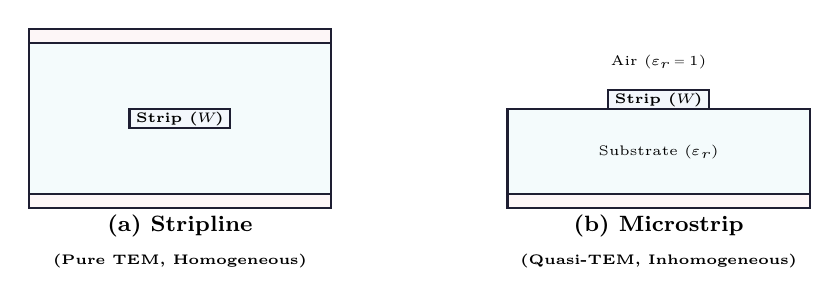
\begin{tikzpicture}[x=1.6cm, y=1.2cm]
  % Stripline Diagram
  \draw[line, fill=hdrteal!30] (0,0) rectangle (2.4,1.6);
  \draw[line, fill=hdrred!40] (0,1.6) rectangle (2.4,1.75); % Top Ground
  \draw[line, fill=hdrred!40] (0,-0.15) rectangle (2.4,0);  % Bottom Ground
  \draw[line, fill=hdrblue!60] (0.8,0.7) rectangle (1.6,0.9); % Center strip
  \node at (1.2,0.8) {\tiny\textbf{Strip ($W$)}};
  \node[align=center] at (1.2,-0.5) {\footnotesize\textbf{(a) Stripline}\\\tiny\textbf{(Pure TEM, Homogeneous)}};
  
  % Microstrip Diagram
  \draw[line, fill=hdrteal!30] (3.8,0) rectangle (6.2,0.9);
  \draw[line, fill=hdrred!40] (3.8,-0.15) rectangle (6.2,0);  % Ground
  \draw[line, fill=hdrblue!60] (4.6,0.9) rectangle (5.4,1.1); % Top strip
  \node at (5.0,1.0) {\tiny\textbf{Strip ($W$)}};
  \node at (5.0,1.4) {\tiny Air ($\varepsilon_r=1$)};
  \node at (5.0,0.45) {\tiny Substrate ($\varepsilon_r$)};
  \node[align=center] at (5.0,-0.5) {\footnotesize\textbf{(b) Microstrip}\\\tiny\textbf{(Quasi-TEM, Inhomogeneous)}};
\end{tikzpicture}
\end{tcolorbox}

% ===============================================================================
% 2. EFFECTIVE DIELECTRIC CONSTANT & IMPEDANCE ANALYSIS
% ===============================================================================
\section{Effective Dielectric Constant (\texorpdfstring{$\varepsilon_{eff}$}{epsilon\_eff}) and Analysis}

\subsection{Concept of Effective Dielectric Constant (\texorpdfstring{$\varepsilon_{eff}$}{epsilon\_eff})}
To simplify the analysis of inhomogeneous microstrip lines, the air-dielectric boundary is replaced by a fictitious homogeneous dielectric medium extending throughout space, characterized by an \textbf{Effective Dielectric Constant ($\varepsilon_{eff}$)}.

\begin{tcolorbox}[formulabox, title={Effective Dielectric Constant ($\varepsilon_{eff}$) Formula}]
  The effective dielectric constant is bounded by $1 < \varepsilon_{eff} < \varepsilon_r$ and is calculated using Schneider's closed-form expression:
  \begin{equation}
    \varepsilon_{eff} = \frac{\varepsilon_r + 1}{2} + \frac{\varepsilon_r - 1}{2} \left[ 1 + 12\frac{h}{W} \right]^{-1/2}
  \end{equation}
  where $W$ is the microstrip width and $h$ is the substrate thickness.
\end{tcolorbox}

\subsection{Guided Wavelength and Phase Velocity}
The phase velocity $v_p$ and guided wavelength $\lambda_g$ in microstrip are given by:
\begin{equation}
  v_p = \frac{c}{\sqrt{\varepsilon_{eff}}} \quad ; \quad \lambda_g = \frac{v_p}{f} = \frac{\lambda_0}{\sqrt{\varepsilon_{eff}}}
\end{equation}

\subsection{Microstrip Characteristic Impedance (\texorpdfstring{$Z_0$}{Z0}) Analysis \& Synthesis}

\begin{enumerate}[leftmargin=*, itemsep=5pt]
  \item \textbf{Analysis Formulas (Given $W/h$ and $\varepsilon_r$, find $Z_0$):}
    \begin{itemize}[leftmargin=*, itemsep=3pt]
      \item For Narrow Strips ($W/h \le 1$):
        \begin{equation}
          Z_0 = \frac{60}{\sqrt{\varepsilon_{eff}}} \ln\left[ 8\frac{h}{W} + 0.25\frac{W}{h} \right]
        \end{equation}
      \item For Wide Strips ($W/h \ge 1$):
        \begin{equation}
          Z_0 = \frac{120\pi}{\sqrt{\varepsilon_{eff}} \left[ \frac{W}{h} + 1.393 + 0.667 \ln\left( \frac{W}{h} + 1.444 \right) \right]}
        \end{equation}
    \end{itemize}

  \item \textbf{Synthesis Formulas (Given target $Z_0$ and $\varepsilon_r$, find required $W/h$):}
    \begin{itemize}[leftmargin=*, itemsep=3pt]
      \item For $W/h < 2$:
        \begin{equation}
          \frac{W}{h} = \frac{8 e^A}{e^{2A} - 2} \quad \text{where } A = \frac{Z_0}{60} \sqrt{\frac{\varepsilon_r+1}{2}} + \frac{\varepsilon_r-1}{\varepsilon_r+1} \left( 0.23 + \frac{0.11}{\varepsilon_r} \right)
        \end{equation}
      \item For $W/h > 2$:
        \begin{equation}
          \frac{W}{h} = \frac{2}{\pi} \left[ B - 1 - \ln(2B-1) + \frac{\varepsilon_r-1}{2\varepsilon_r} \left( \ln(B-1) + 0.39 - \frac{0.61}{\varepsilon_r} \right) \right]
        \end{equation}
        where $B = \frac{377\pi}{2 Z_0 \sqrt{\varepsilon_r}}$.
    \end{itemize}
\end{enumerate}

\subsection{Stripline Characteristic Impedance Formula}
For a symmetrical stripline with ground plane spacing $b$ and effective strip width $W_e$:
\begin{equation}
  Z_{0,\text{strip}} = \frac{30\pi}{\sqrt{\varepsilon_r}} \frac{b}{W_e + 0.441b} \quad \text{where } W_e = W \text{ for } t/b \to 0
\end{equation}

\begin{tcolorbox}[examplebox, title={Worked Numerical: Microstrip Design \& Wavelength Calculation}]
  \textbf{Problem:} A microstrip line is printed on an Alumina substrate ($\varepsilon_r = 9.8$, $h = 0.635\text{ mm}$). If the width-to-height ratio is $W/h = 1.0$, calculate:
  \begin{enumerate}[label=(\alph*), noitemsep]
    \item The effective dielectric constant $\varepsilon_{eff}$.
    \item The characteristic impedance $Z_0$.
    \item The guided wavelength $\lambda_g$ at $10\text{ GHz}$.
  \end{enumerate}
  \tcblower
  \textbf{Solution:}
  \begin{enumerate}[label=(\alph*), itemsep=4pt]
    \item Calculate $\varepsilon_{eff}$ using $W/h = 1.0$:
      \begin{equation}
        \begin{aligned}
          \varepsilon_{eff} &= \frac{9.8 + 1}{2} + \frac{9.8 - 1}{2} \left[ 1 + 12(1) \right]^{-1/2} \\
          &= 5.4 + 4.4 \left[ 13 \right]^{-1/2} = 5.4 + \frac{4.4}{3.6055} \\
          &= 5.4 + 1.2203 = 6.6203
        \end{aligned}
      \end{equation}
    \item Since $W/h = 1.0 \le 1$, use the narrow strip formula for $Z_0$:
      \begin{equation}
        \begin{aligned}
          Z_0 &= \frac{60}{\sqrt{6.6203}} \ln\left[ 8(1) + 0.25(1) \right] \\
          &= \frac{60}{2.573} \ln(8.25) = 23.319 \times 2.1102 \\
          &= 49.21\text{ }\Omega \approx 50\text{ }\Omega
        \end{aligned}
      \end{equation}
    \item Free-space wavelength $\lambda_0 = \frac{c}{f} = \frac{3 \times 10^8\text{ m/s}}{10 \times 10^9\text{ Hz}} = 30\text{ mm}$.
      \begin{equation}
        \lambda_g = \frac{\lambda_0}{\sqrt{\varepsilon_{eff}}} = \frac{30\text{ mm}}{\sqrt{6.6203}} = \frac{30}{2.573} = 11.66\text{ mm}
      \end{equation}
  \end{enumerate}
\end{tcolorbox}

% ===============================================================================
% 3. LOSSES, DISPERSION, AND DISCONTINUITIES
% ===============================================================================
\section{Losses, Dispersion, and Discontinuities in Microstrip}

\subsection{Microstrip Attenuation \& Loss Mechanisms}
Total attenuation constant $\alpha_{total} = \alpha_c + \alpha_d + \alpha_r$ ($\text{Np/m}$ or $\text{dB/m}$):

\begin{itemize}[leftmargin=*, itemsep=4pt]
  \item \textbf{Conductor Loss ($\alpha_c$):} Skin effect causes current to crowd within skin depth $\delta = \sqrt{\frac{1}{\pi f \mu \sigma}}$ along lower surface edges:
    \begin{equation}
      \alpha_c \approx \frac{8.686 R_s}{Z_0 W} \text{ dB/m} \quad \text{where } R_s = \sqrt{\frac{\pi f \mu}{\sigma}} \text{ (Surface Resistance)}
    \end{equation}
  \item \textbf{Dielectric Loss ($\alpha_d$):} Caused by substrate dipole relaxation loss:
    \begin{equation}
      \alpha_d = 27.3 \frac{\varepsilon_r}{\sqrt{\varepsilon_{eff}}} \frac{\varepsilon_{eff}-1}{\varepsilon_r-1} \frac{\tan\delta}{\lambda_0} \quad \text{dB/m}
    \end{equation}
  \item \textbf{Radiation Loss ($\alpha_r$):} At high frequencies, microstrip open boundaries act as long slot radiators emitting RF energy into space.
\end{itemize}

\subsection{Microstrip Discontinuities}
Physical transitions in microstrip layouts alter local electric and magnetic field distributions, generating parasitic reactances.

\par\vspace{6pt}\noindent
\begingroup
\renewcommand{\arraystretch}{1.4}%
\begin{tabularx}{\linewidth}{|>{\raggedright\arraybackslash\bfseries}p{3.2cm}|Y|Y|}
\hline
\textbf{Discontinuity Type} & \textbf{Physical Origin} & \textbf{Equivalent Circuit Model \& Mitigation} \\
\hline
Open-End Line & Fringing electric fields extend past strip termination into air & Shunt end capacitance $C_{oc}$, equivalent to extra length $\Delta l = 0.412 h \frac{\varepsilon_{eff}+0.3}{\varepsilon_{eff}-0.258} \frac{W/h+0.264}{W/h+0.8}$. \\
\hline
Step-Change in Width & Sudden width transition $W_1 \to W_2$ disrupts current distribution & Series inductance $L_s$ and shunt capacitance $C_s$. \\
\hline
Right-Angle Bend ($90^\circ$) & Current crowding at inner corner; excess charge at outer corner & Series inductance $L_b$ and shunt capacitance $C_b$. Mitigated by $45^\circ$ Mitred Bend ($M = 52 + 65 e^{-1.35 W/h}\%$ metal removal). \\
\hline
T-Junction / Cross & Junction of orthogonal microstrip branches & Equivalent $T$-network of series inductances and shunt capacitance. \\
\hline
\end{tabularx}
\endgroup

% ===============================================================================
% QUICK REVISION PAGE
% ===============================================================================
\newpage
\begin{center}
  {\large\bfseries\color{myred} Quick Revision --- Module 2}\\[3pt]
  {\small\color{mydark} Planar Transmission Lines-I (Stripline \& Microstrip) $|$ OE-EC804B}
\end{center}
\noindent{\color{myred}\rule{\linewidth}{1.2pt}}
\vspace{4pt}

\begin{tcolorbox}[formulabox, title={\textbf{Key Concepts and Metrics at a Glance}}]
\renewcommand{\arraystretch}{1.35}
\begin{tabularx}{\linewidth}{>{\raggedright\arraybackslash\bfseries}p{4.5cm} X}
Effective Dielectric $\varepsilon_{eff}$ & $\varepsilon_{eff} = \frac{\varepsilon_r+1}{2} + \frac{\varepsilon_r-1}{2} \left[1 + 12\frac{h}{W}\right]^{-1/2} \quad (1 < \varepsilon_{eff} < \varepsilon_r)$ \\[4pt]
Phase Velocity \& Wavelength & $v_p = \frac{c}{\sqrt{\varepsilon_{eff}}} \quad ; \quad \lambda_g = \frac{\lambda_0}{\sqrt{\varepsilon_{eff}}}$ \\[4pt]
Stripline Propagation & Pure TEM mode ($E_z=0, H_z=0$) due to symmetrical homogeneous dielectric. \\[4pt]
Microstrip Propagation & Inhomogeneous Quasi-TEM mode ($E_z, H_z \ne 0$) due to air-substrate boundary. \\[4pt]
Mitred Bend Optimal Cut & $M = \frac{x}{d\sqrt{2}} \times 100\% = 52 + 65 e^{-1.35 W/h}\%$ removes $90^\circ$ corner capacitance. \\
\end{tabularx}
\end{tcolorbox}

\begin{tcolorbox}[defbox, title={\textbf{One-Line Definitions}}]
  \begin{itemize}[leftmargin=*, noitemsep]
    \item \textbf{Quasi-TEM Mode:} Hybrid electromagnetic wave in non-homogeneous media possessing tiny longitudinal field components.
    \item \textbf{Fringing Fields:} Electric field lines extending into the air region surrounding microstrip edges.
    \item \textbf{Mitred Bend:} A $45^\circ$ chamfered microstrip bend removing excess corner capacitance to maintain $50\text{ }\Omega$ matching.
    \item \textbf{Microstrip Dispersion:} Frequency-dependent variation of $\varepsilon_{eff}(f)$ causing phase velocity to decrease at high frequencies.
  \end{itemize}
\end{tcolorbox}

\begin{tcolorbox}[exambox, title={\textbf{Frequently Asked / Viva Questions}}]
  \begin{enumerate}[topsep=0pt, label=\textbf{Q\arabic*.}, itemsep=5pt]
    \item \Q{Why does a microstrip line support a Quasi-TEM mode instead of a pure TEM mode?}
    Because the electromagnetic field exists in two different media (dielectric substrate and air), causing phase velocity mismatch that induces small longitudinal $E_z$ and $H_z$ components.

    \item \Q{Why does a stripline support a pure TEM mode?}
    Because the conductor is completely enclosed inside a single homogeneous dielectric bounded by two ground planes.

    \item \Q{What is the Effective Dielectric Constant ($\varepsilon_{eff}$) of a microstrip?}
    A weighted average dielectric constant of air and substrate representing a fictitious homogeneous medium supporting the same wave velocity.

    \item \Q{How does characteristic impedance ($Z_0$) vary with strip width $W$?}
    As strip width $W$ increases, capacitance increases and characteristic impedance $Z_0$ decreases ($Z_0 \propto 1/W$).

    \item \Q{Explain the physical significance of an open-end microstrip discontinuity.}
    Fringing fields at the open termination store electric energy, behaving as a shunt capacitor $C_{oc}$ that increases the line's effective length by $\Delta l$.

    \item \Q{Why are right-angle microstrip bends mitred (chamfered)?}
    A $90^\circ$ sharp bend creates excess capacitance at the outer corner. Mitring removes $50\%$ to $60\%$ of the corner metal, eliminating reflections.

    \item \Q{What are the main loss mechanisms in microstrip lines?}
    Conductor loss $\alpha_c$ (skin effect), dielectric loss $\alpha_d$ (substrate dissipation), and radiation loss $\alpha_r$ (open boundary power leakage).

    \item \Q{Differentiate between Stripline and Microstrip in terms of isolation.}
    Stripline provides superior shielding against crosstalk due to dual ground planes. Microstrip suffers higher radiation loss due to its open top boundary.

    \item \Q{How does dispersion affect microstrip performance at high frequencies?}
    As frequency increases, fields become more confined inside the substrate, increasing $\varepsilon_{eff}(f)$ towards $\varepsilon_r$ and causing dispersion (signal distortion).

    \item \Q{What is the typical value of $\varepsilon_{eff}$ relative to $\varepsilon_r$?}
    $\varepsilon_{eff}$ is strictly bounded by $1 < \varepsilon_{eff} < \varepsilon_r$, typically around $0.65\varepsilon_r$ for standard microstrips.
  \end{enumerate}
\end{tcolorbox}

\end{document}
